\paragraph{}En esta página se le muestra al usuario el total de los microcontralodores, tanto en unidades como en precio, que ha ido añadiendo a su carro de la compra durante su visita a la página web $\mu$Search, permitiéndole al usario modificar dichas unidades de cada microcontrolador elegido y finalmente generar un presupuesto o factura.

\begin{figure}[h!]
	\centering
	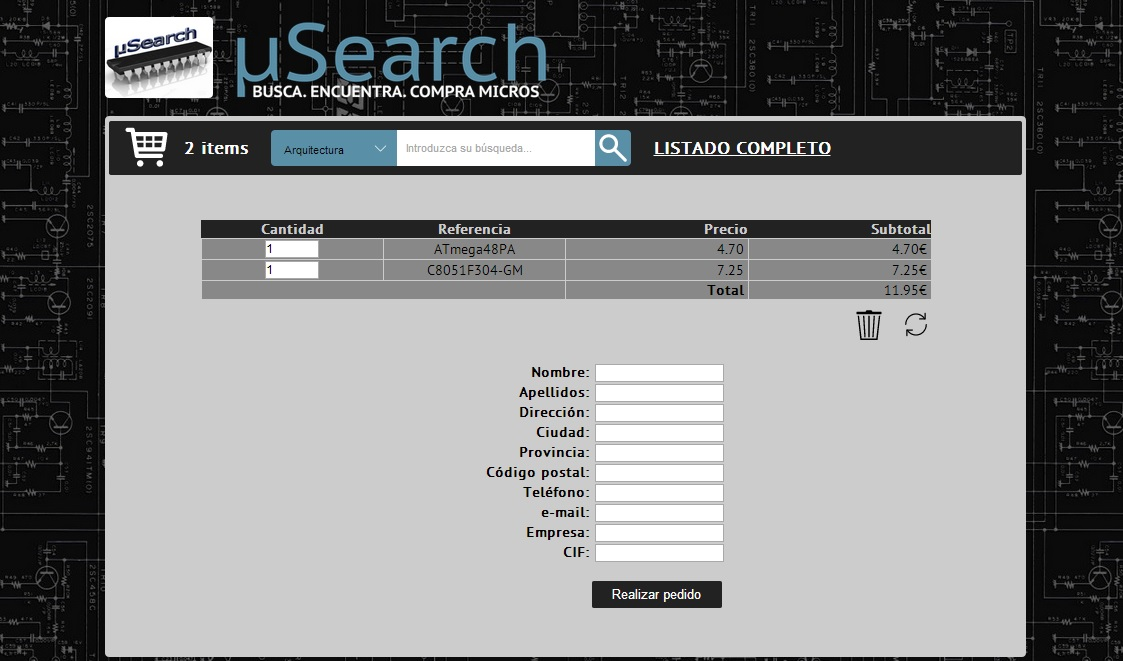
\includegraphics[width=0.75\textwidth]{img/carrito}
	\caption{Carrito de la compra.}
	\label{fig:carrito}
\end{figure}

Como en todas las demás páginas del sitio web, pulsando en cualquiera de los logotipos del catálogo $\mu$Search, el sistema redirigirá al usuario a la página inicial del catálogo.

\paragraph{}Debajo de los dos logotipos anteriormente citados, se encuentran dos iconos en la cabecera de la página que permiten las siguientes acciones:

\begin{itemize}
	\item \textbf{Carrito de la compra:} A su lado, aparece también el número de artículos que han sido introducidos en el mismo, pulsando sobre este icono se vuelve a cargar la página actual. Volver a cargar la página actual puede ser útil en el caso de que se haya modificado la cantidad de uno o varios artículos del carrito y se quiera deshacer estos cambios sin que tengan ningún efecto en el precio final de la compra.

	\item \textbf{Búsqueda:} Desde esta sección de la cabecera, el usuario puede realizar búsquedas sobre el catálogo de microcontroladores en base a cualquiera de las diferentes características de un microcontrolador (Arquitectura, Frecuencia, Flash, RAM). Simplemente se debe seleccionar una de las características de la lista despegable, introducir el texto a buscar y pulsar sobre el icono de búsqueda.
	El usuario será redirigido a una página donde se le mostrará el resultado de la búsqueda en forma de lista de microcontroladores.

	\item \textbf{Listado Completo:} Pulsando sobre este botón/icono el sistema redirige al usuario a la página en la que se listan todos los elementos disponibles en el catálogo de microcontroladores.
\end{itemize}

A continuación, se encuentra en forma de tabla el listado de los microcontroladores que el usuario ha ido añadiendo al carrito de la compra. Este listado, esta compuesto por cuatro columnas: 
\begin{itemize}
	\item \textbf{Cantidad:} La cantidad de unidades de cada elemento añadido al carrito de la compra es un campo modificable que permite	solicitar más o menos unidades de ese elemento. Para que estos cambios tengan efecto es necesario actualizar el listado como se explica en el apartado siguiente. Si el usuario pulsa la tecla \textit{Enter} del teclado, teniendo todavía activo el campo de la cantidad de un elemento, también implica aceptar los cambios realizados hasta el momento.
	
	\item \textbf{Referencia:} Es el código del fabricante que identifica a cada elemento del catálogo, cada microcontrolador
	tiene una referencia única.
	
	\item \textbf{Precio:} Es el precio que tiene una unidad de un microcontrolador específico.

	\item \textbf{Subtotal:} Es el resultado de multiplicar el número de unidades solicitadas de un microcontrolador por el precio que tiene cada unidad. Hay tantos subtotales como elementos en el carrito de la compra.
\end{itemize}

Debajo del listado de los elementos del carrito de la compra, se encuentran dos botones que pueden tener efecto sobre todos los microcontroladores solicitados:
\begin{itemize}
	\item \textbf{Actualizar:}  Este botón hay que pulsarlo después de modificar una o varias cantidades de los elementos del 
	carrito de la compra. Es el que permite que dichos cambios tengan efecto. Se puede observar cómo cambia el precio total de la compra.
	Además, si alguna nueva cantidad tiene un valor de 0, el elemento que tenga dicha cantidad será eliminado del carrito de la compra.
	
	\item \textbf{Vaciar:}  Pulsando sobre este botón se vacía completamente el carrito de la compra.
\end{itemize}

\paragraph{}Antes de finalizar el pedido, hay disponible un formulario que el cliente debe rellenar con sus datos de contacto para poder generar correctamente la factura asociada al pedido que se quiere realizar. Todos los campos son obligatorios excepto el nombre y CIF de la empresa.

\paragraph{}Finalmente, una vez que el cliente ha revisado que todos los datos relativos al pedido (cantidades, referencias, precios, datos personales, etc.) son correctos hay que pulsar sobre el botón \textbf{\textit{''Realizar Pedido''}} para que el sistema genere la factura asociada a dicho pedido.